\documentclass[11pt,landscape]{exam}
\usepackage[margin=0.3in]{geometry}
\usepackage{multicol,tikz,graphicx}
\usetikzlibrary{shadings,decorations.pathmorphing,arrows.meta,patterns}




\begin{document}

\newcommand{\content}{


\section*{Reflection}
\begin{itemize}
  \item light \fillin[bounces][7em] off of a new medium
  \item The angle of incidence is \fillin[equal][5em] to the angle of Reflection
\end{itemize}

\begin{center}
  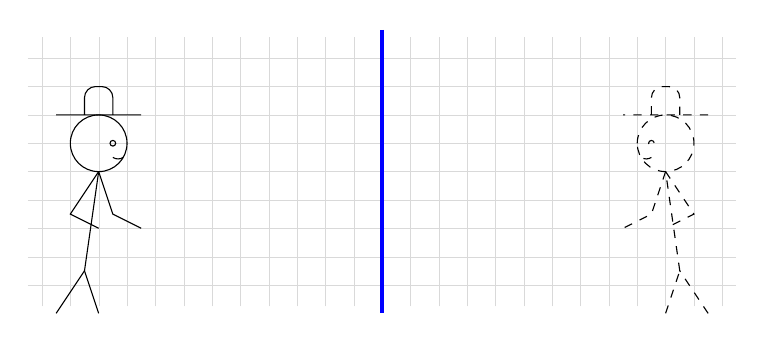
\begin{tikzpicture}[scale=0.9]
      \draw[gray!30,ultra thin] (-5,0.1) grid[step=0.4] (5,3.9);


    \def\person{
      \begin{scope}[scale=2, shift={(-2,0)}]
        \draw (0,1.2) circle (0.2);
        \coordinate (waste) at (-.1,.3);
        \coordinate (neck) at (0,1);
        \draw (waste) -- (neck);
        \draw (-.3,0) -- (waste);
        \draw (0,0) -- (waste);
        \draw (neck) -- ++(.1,-.3) -- ++(.2,-.1);
        \draw (neck) -- ++(-.2,-.3) -- ++(.2,-.1);

        \draw[rounded corners] (neck) ++(-.3,.4) -- +(.6,0)
          ++(.2,0) -- ++(0,0.2) -- ++(0.2,0) -- ++(0,-0.2);

        \path (0,1.2) ++(-30:0.2) coordinate (smile);

        \draw (neck) ++(0.1,0.2) circle (0.02)
            ++(0,-0.1) to[bend right] (smile);
      \end{scope}
    }

    \draw[ultra thick, blue] (0,4) -- (0,0);

    \begin{scope}
      \person
    \end{scope}
    \begin{scope}[xscale=-1,yscale=1, dashed]
      \person
    \end{scope}

  \end{tikzpicture}
\end{center}


\paragraph{Diffuse and Specular Reflection} \hfill

\vspace{4em}

\begin{center}
    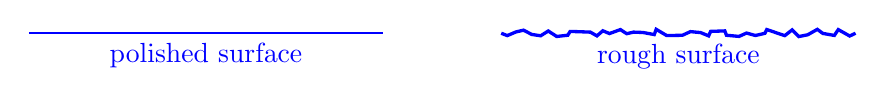
\begin{tikzpicture}
    \draw[blue,thick] (0,0) -- ++(4.5,0) node[midway,below] {polished surface};
    \draw[blue,very thick,decorate,decoration={random steps,segment length=0.1cm,amplitude=.05cm}] 
      (6,0) -- ++(4.5,0) node[midway,below] {rough surface};
  \end{tikzpicture}
\end{center}


\section*{Refraction}

\vspace{4em}

\begin{center}
    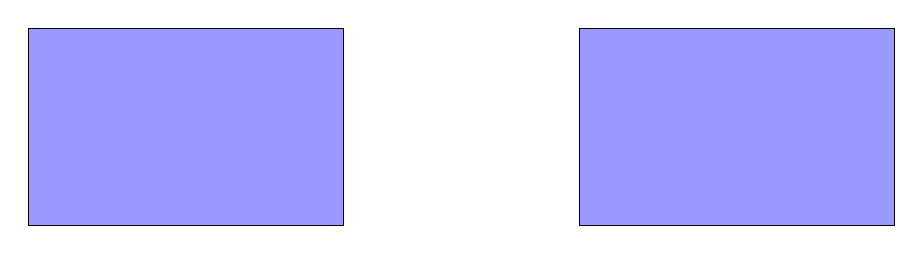
\begin{tikzpicture}
    \draw[fill=blue!40] (0,0) rectangle ++(4,2.5);
    \draw[fill=blue!40] (7,0) rectangle ++(4,2.5);
  \end{tikzpicture}
\end{center}


\begin{itemize}
  \item when light slows down, it bends \fillin[toward][12em] normal.
  \item when light speeds up, it bends \fillin[away from][12em] normal.
  \item \textbf{total internal reflection} occurs when the angle is \fillin[too large][9em] for refraction to occur and the light \fillin[reflects][12em] instead.
\end{itemize}

\vspace{5em}

}




\begin{multicols}{2}

\content

\columnbreak

\content

\end{multicols}



\end{document}